% pgfplots oracle fixture (hand-written): two axes in one picture, the second
% placed relative to the first by name.
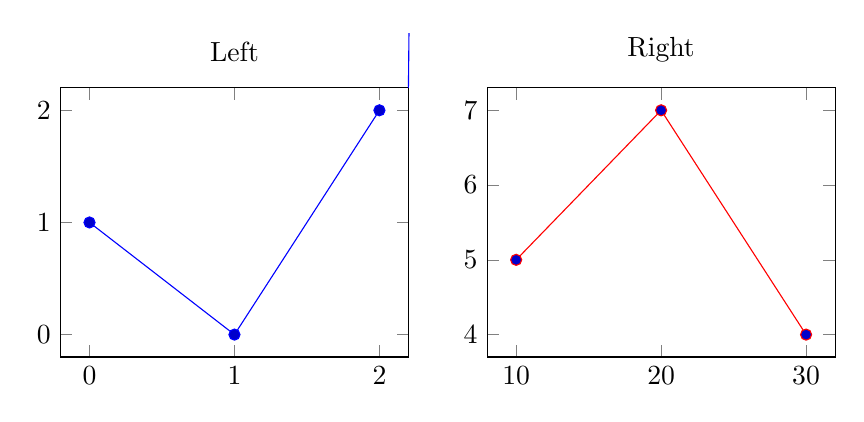
\begin{tikzpicture}
\begin{axis}[name=left, width=6cm, height=5cm, title={Left}]
\addplot coordinates {(0,1) (1,0) (2,2)};
\end{axis}
\begin{axis}[at={(left.south east)}, xshift=1cm, width=6cm, height=5cm, title={Right}]
\addplot+[red] coordinates {(10,5) (20,7) (30,4)};
\end{axis}
\draw[blue] (left.north east) -- (left.outer north east);
\end{tikzpicture}
